        
            \begin{naloga}
                Dve stranici trikotnika merita $2$ in $7$ enot. 
                Zapišite interval vrednosti za dolžino tretje stranice tega trikotnika.
            \end{naloga}

            \begin{naloga}
                Ali obstaja trikotnik, katerega dolžine stranic so rešitve sistema enačb:
                \begin{align*}
                    a+b+c&=16 \\ a-c&=2 \\ a+b&=13 .
                \end{align*}
            \end{naloga}

            \begin{naloga}
                Za katere vrednosti števila $x$ obstaja trikotnik s stranicami dolžin $x+7$, $2x+2$ in $3x-1$?
            \end{naloga}
        

        
                \begin{naloga}
                    Izračunajte velikosti kotov $\alpha$ in $\beta$.
                    \begin{figure}
                        \centering
                        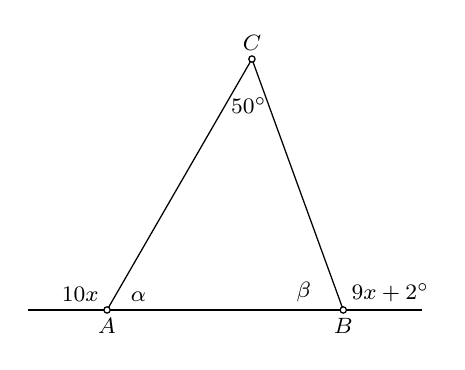
\begin{tikzpicture}
                            % \clip (0,0) rectangle (14.000000,10.000000);
                            {\footnotesize

                            % Drawing line A B
                            \draw [line width=0.016cm] (1.000000,1.500000) -- (1.960000,1.500000);%
                            \draw [line width=0.016cm] (2.040000,1.500000) -- (4.960000,1.500000);%
                            \draw [line width=0.016cm] (5.040000,1.500000) -- (6.000000,1.500000);%

                            % Drawing segment A C
                            \draw [line width=0.016cm] (2.020000,1.534641) -- (3.820022,4.652371);%

                            % Drawing segment B C
                            \draw [line width=0.016cm] (4.986319,1.537588) -- (3.853703,4.649424);%

                            % Marking point A by circle
                            \draw [line width=0.016cm] (2.000000,1.500000) circle (0.040000);%
                            \draw (2.000000,1.500000) node [anchor=north] { $A$ };%

                            % Marking point B by circle
                            \draw [line width=0.016cm] (5.000000,1.500000) circle (0.040000);%
                            \draw (5.000000,1.500000) node [anchor=north] { $B$ };%

                            % Marking point C by circle
                            \draw [line width=0.016cm] (3.840022,4.687012) circle (0.040000);%
                            \draw (3.840022,4.687012) node [anchor=south] { $C$ };%

                            % Marking point \alpha
                            \draw (2.400000,1.500000) node [anchor=south] { $\alpha$ };%

                            % Marking point \beta
                            \draw (4.500000,1.500000) node [anchor=south] { $\beta$ };%

                            % Marking point {10x}
                            \draw (2.000000,1.500000) node [anchor=south east] { ${10x}$ };%

                            % Marking point {9x+2^\circ}
                            \draw (5.000000,1.500000) node [anchor=south west] { ${9x+2^\circ}$ };%

                            % Marking point {50^\circ}
                            \draw (3.800000,4.300000) node [anchor=north] { ${50^\circ}$ };%
                            }
                        \end{tikzpicture}

                    \end{figure}
                \end{naloga}


                \begin{naloga}
                    Premici $p$ in $q$ sta vzporedni.
                    Izračunajte velikosti kotov $\alpha$, $\beta$ in $\gamma$.
                    \begin{figure}
                        \centering
                        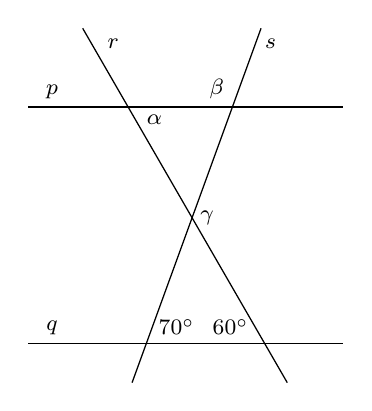
\begin{tikzpicture}
                            % \clip (0,0) rectangle (14.000000,10.000000);
                            {\footnotesize

                            % Drawing line a
                            \draw [line width=0.016cm] (1.000000,1.500000) -- (5.000000,1.500000);%

                            % Drawing line b
                            \draw [line width=0.016cm] (1.000000,4.500000) -- (5.000000,4.500000);%

                            % Drawing line c
                            \draw [line width=0.016cm] (2.318015,1.000000) -- (3.955881,5.500000);%

                            % Drawing line d
                            \draw [line width=0.016cm] (4.288675,1.000000) -- (1.690599,5.500000);%

                            % Marking point p
                            \draw (1.300000,4.500000) node [anchor=south] { $p$ };%

                            % Marking point q
                            \draw (1.300000,1.500000) node [anchor=south] { $q$ };%

                            % Marking point r
                            \draw (1.900000,5.300000) node [anchor=west] { $r$ };%

                            % Marking point s
                            \draw (3.900000,5.300000) node [anchor=west] { $s$ };%

                            % Marking point \gamma
                            \draw (3.079989,3.093506) node [anchor=west] { $\gamma$ };%

                            % Marking point \alpha
                            \draw (2.400000,4.500000) node [anchor=north west] { $\alpha$ };%

                            % Marking point \beta
                            \draw (3.591911,4.500000) node [anchor=south east] { $\beta$ };%

                            % Marking point {70^\circ}
                            \draw (2.550000,1.500000) node [anchor=south west] { ${70^\circ}$ };%

                            % Marking point {60^\circ}
                            \draw (3.900000,1.500000) node [anchor=south east] { ${60^\circ}$ };%
                            }
                        \end{tikzpicture}

                    \end{figure}
                \end{naloga}
                
        

        
            \begin{naloga}
                Izračunajte velikosti vseh notranjih in zunanjih kotov trikotnika $\triangle ABC$, 
                če je vsota velikosti dveh zunanjih kotov $\alpha'+\gamma'=230^\circ$, vsota velikosti dveh notranjih kotov pa $\alpha+\beta=70^\circ$.
            \end{naloga}

            \begin{naloga}
                Izračunajte velikosti vseh notranjih in zunanjih kotov trikotnika $\triangle ABC$, 
                če je vsota velikosti dveh zunanjih kotov $\alpha'+\beta'=234^\circ$, razlika velikosti dveh notranjih kotov pa $\alpha-\beta=28^\circ$.
            \end{naloga}

        


        
            \begin{naloga}
                Narišite trikotnik s podatki:
                \begin{itemize}
                    \item $a=4~cm$, $b=5~cm$ in $c=7~cm$,
                    \item $a=4~cm$, $b=6~cm$ in $\beta=60^\circ$,
                    \item $a=4~cm$, $b=4.5~cm$ in $t_a=4~cm$,
                    \item $b=4~cm$, $t_b=5~cm$ in $\gamma=105^\circ$,
                    \item $v_a=4~cm$, $t_c=2.5~cm$ in $\beta=30^\circ$,
                    \item $b=5~cm$, $v_a=2~cm$ in $\beta=30^\circ$,
                    \item $a+b+c=13~cm$, $v_c=3~cm$ in $\alpha=60^\circ$,
                    \item $a+b=7~cm$, $\alpha=45^\circ$ in $v_b=4~cm$.
                \end{itemize}
            \end{naloga}
        
